\documentclass[a4paper, 12pt]{article}
\usepackage[T1]{fontenc}
\usepackage{lmodern}
\usepackage{pdfpages}
\usepackage{color}
\usepackage{amsfonts}
\usepackage{epstopdf}
\usepackage{matlab}
%\documentclass{book}
\usepackage{blindtext}
\usepackage{hyperref}
\usepackage[brazil]{babel}
\usepackage{amssymb}
\usepackage[utf8]{inputenc}
\usepackage{amsmath}
\usepackage{indentfirst}
\usepackage{graphicx}
\usepackage{multicol,lipsum}
\usepackage[a4paper,
top=3cm, left=3cm, bottom=3cm, right=3cm]{geometry}
\usepackage{setspace}
\usepackage{multirow}
\usepackage{float}
\usepackage[dvipsnames]{xcolor}
\usepackage[table]{xcolor}
%\usepackage{pdflscape}
\usepackage[DIV=15]{typearea}
\usepackage[nottoc]{tocbibind}
\usepackage[sort,numbers]{natbib}
%\usepackage{cite}
\usepackage{matlab}

\usepackage[utf8]{inputenc}
\usepackage[T1]{fontenc}
\usepackage{lmodern}
\usepackage{graphicx}
\usepackage{color}
\usepackage{hyperref}
\usepackage{amsmath}
\usepackage{amsfonts}
\usepackage{epstopdf}
\usepackage[table]{xcolor}
\usepackage{matlab}


\documentclass[letterpaper]{article}
% bib pack %%%%%%%%%%%%%%%%%%%%%%%%%%%%%%%%%%%%%%%%%%%%%%%%%%%%%%%%%%%%%%%%%%%%%
\usepackage[utf8]{inputenc}
\usepackage{geometry}
    \geometry{left=3cm,right=2cm,top=2cm,bottom=2cm}
%
\usepackage[spanish]{babel}
%
\usepackage[fixlanguage]{babelbib}
    \bibliographystyle{babunsrt}
%
\usepackage{url}

\begin{document}
%\maketitle

\begin{titlepage}
	\begin{center}
		

\vspace{10pt}
%\begin{figure}[H][!ht]
%\centering
%
\includegraphics{puc-rio-logo.png}

%\end{figure}
\begin{figure}[!ht]
\centering

\includegraphics{images/puc-rio-logo.png}
\end{figure}
\huge{Fundamentos de Mecatrônica}
        \vspace{70pt}
        
		\textbf{ENG1731}
		\textbf{\large{\\ }}
		
		\vspace{30pt}
		\textbf{\small{\\Lista 05}}
		\vspace{75pt}
		
	\end{center}
	
	\begin{flushleft}
		\begin{tabbing}
		Aluno(a)\qquad\qquad\=\>Paloma Fernanda Loureiro Sette - 1621595\\
			
			Professor(a)\>João Carlos Virgolino Soares\\
	\end{tabbing}
		  
	\end{flushleft}
	\begin{center}
		%\vspace{\fill}
		\vspace{215pt}
		Rio de Janeiro, 26 de Maio de 2023
	\end{center}
\end{titlepage}
%%%%%%%%%%%%%%%%%%%%%%%%%%%%%%%%%%%%%%%%%%%%%%%%%%%%%%%%%%%
\newpage
\tableofcontents
\thispagestyle{empty}

\newpage
\pagenumbering{arabic}

\newpage

%\newcommand{\listequationsname}{Lista de Equações}
%\newlistof{myequations}{equ}{\listequationsname}
%\newcommand{\myequations}[1]{%
%\addcontentsline{equ}{myequations}{\protect\numberline{\theequation}#1}\par}

%\listofmyequations
\newpage


\newpage

\listoffigures
\thispagestyle{empty}

\newpage
%%%%%%%%%%%%%%%%%%%%%%%%%%%%%%%%%%%%%%%%%%%%%%%%%%%%%%%%%
%%%%%%%%%%%%%%%%%%%%%%%%%%%%%%%%%%%%%%%%%%%%%%%%%%%

\newpage

\thispagestyle{empty}

%%%%%%%%%%%%%%%%%%%%%%%%%%%%%%%%%%%%%%%%%%%%%%%%%%%%%%%%%%%%%%%%%%%%%%%
\newpage
\section{Introdução}
Este relatório refere-se ao quinto trabalho da disciplina de Fundamentos de Mecatrônica, ENG1731, de 2023.1. \\

Para estudo do servomotor, consideraremos os parâmetros relativos à parte de controle do servomotor, como potenciômetro, entrada, saída etc. Para a modelagem matemática, consideraremos o circuito do motor DC, o par de engrenagens e a carga. Embora já tenhamos visto o motor DC com carga, agora, no caso do servomotor, é acrescentado um par de engrenagens intermediando estes elementos. 

Trataremos da simulação de um sistema mecânico do servomotor FEETECH RC Model, cujo datasheet é apresentado na página seguinte.\\

%%%%%%%%%%%%%%%%%%%%%%%%%%%%%%%%%%%%%%%%%%%%%%%%%%%%%%%%%%%%%%%%%%%%%%
\newpage
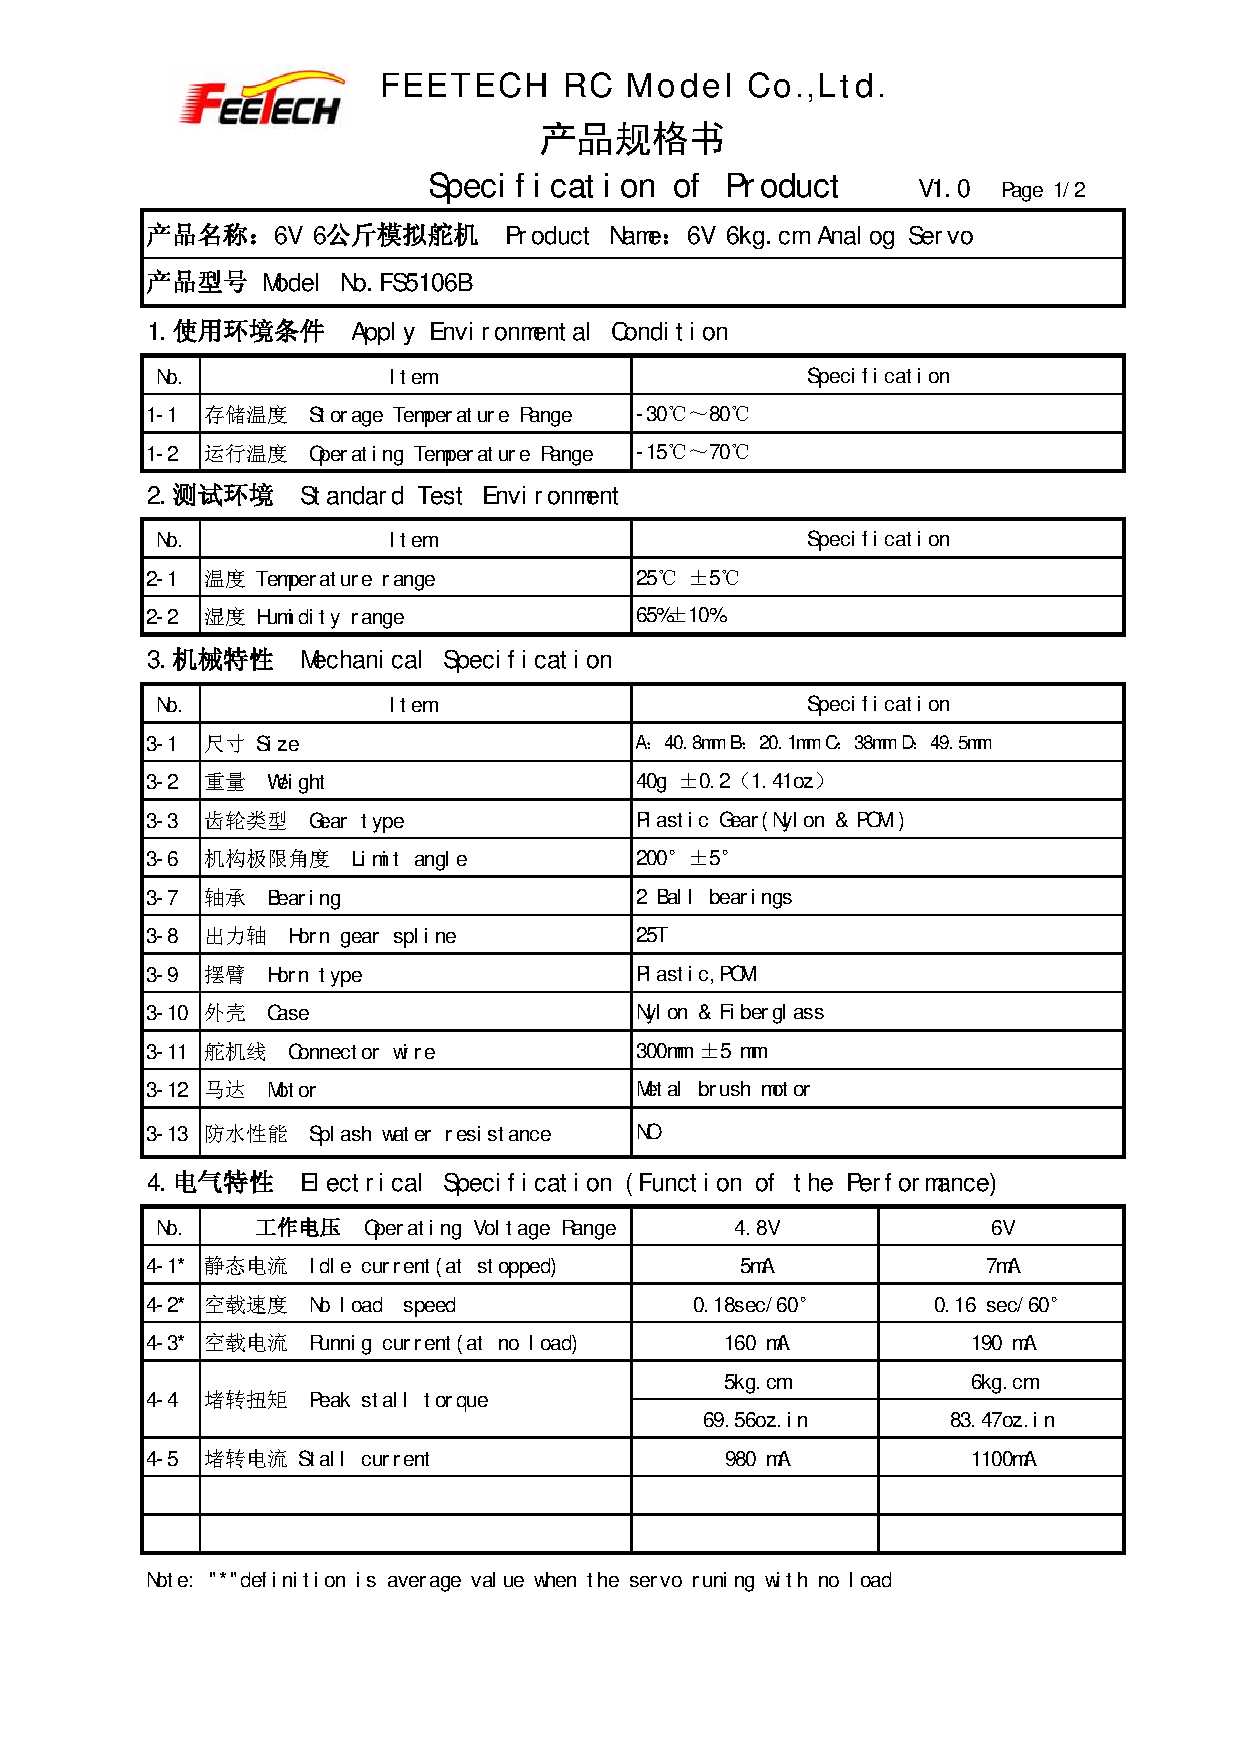
\includepdf[pages={1, 2}, pagecommand={\section{Anexo}}, 
    scale=0.9, 
    offset=0mm -10mm, 
    pagecommand={\thispagestyle{plain}},
    clip, 
    trim=10mm 10mm 10mm 10mm,
    center]{FS5106B specs.pdf}
%%%%%%%%%%%%%%%%%%%%%%%%%%%%%%%%%%%%%%%%%%%%%%%%%%%%%%%%%%%%%%%%%%%%%%


\newpage

\section{Questão 01}
\textbf{Pesquisar e selecionar na internet um \textit{datasheet} de servomotor que contenha os parâmetros vistos nas aulas.} \\

\subsection{Parâmetros}
\textbf{Selecione no datasheet os parâmetros necessários para simular o comportamento do servomotor.} \\



%%%%%%%%%%%%%%%%%%%%%%%%%%%%%%%%%%%%%%%%%%%%%%%%%%%%%%%%%%%%%%%%%%%%%%%
\newpage
\subsection{Comportamento Dinâmico}
\textbf{Simule o comportamento dinâmico do motor escolhido no Simscape ou Simulink utilizando os parâmetros do datasheet.} \\
 
%%%%%%%%%%%%%%%%%%%%%%%%%%%%%%%%%%%%%%%%%%%%%%%%%%%%%%%%%%%%%%%%%%%%%%%%%
\newpage
\subsection{Sinal de Duty Cycle}
\textbf{Crie um sinal de duty cycle usando o bloco \textit{Signal Builder}.}\\


%%%%%%%%%%%%%%%%%%%%%%%%%%%%%%%%%%%%%%%%%%%%%%%%%%%%%%%%%%%%%%%%%%%%%%%%
\newpage
\subsection{Script no MATLAB}
\textbf{Crie um script no MATLAB para definir as variáveis, receber os dados do Simulink e plotar a
velocidade angular, ângulo de saída e \textit{duty cycle}.}

%%%%%%%%%%%%%%%%%%%%%%%%%%%%%%%%%%%%%%%%%%%%%%%%%%%%%%%%%%%%%%%%%%%%%%%%%%%%
\newpage
\subsection{Explicando os resultados}


%%%%%%%%%%%%%%%%%%%%%%%%%%%%%%%%%%%%%%%%%%%%%%%%%%%%%%%%%%%%%%%%%%%%%%%%%
\newpage
\section{Questão 02}
\subsection{(a) }
\textbf{Explique as principais diferenças entre um motor de passo e um servo motor, em termos de
funcionamento e performance.}\\

Os motores de passo e os servo motores apresentam diferenças significativas em termos de funcionamento e desempenho. Podemos explorar as principais diferenças entre eles:\\

\subsubsection{Funcionamento:}\\
\textbf{Motor de Passo:} Os motores de passo são motores de malha aberta, ou seja, não possuem feedback de posição. Eles são projetados para girar em passos discretos, controlados por pulsos elétricos aplicados em suas bobinas. Cada pulso resulta em um ângulo de rotação fixo, conhecido como passo. Os motores de passo são ideais para aplicações em que a precisão de posicionamento é crucial.\\

\textbf{Servo Motor:} Os servo motores são motores de malha fechada, o que significa que possuem um feedback de posição para controle preciso. Eles consistem em um motor de corrente contínua (DC) acoplado a um dispositivo de feedback, como um encoder. O controlador do servo motor monitora constantemente a posição real e ajusta o sinal de controle para alcançar e manter a posição desejada. Os servo motores são adequados para aplicações em que o controle de posição e velocidade é fundamental.\\

\subsubsection{Controle:}

\textbf{Motor de Passo:} O controle de um motor de passo é relativamente simples. A rotação é realizada enviando sequências de pulsos para as bobinas do motor. A frequência e o número de pulsos determinam a velocidade e a posição do motor. É possível alcançar um controle preciso de posição, mas a velocidade de rotação é limitada e o torque diminui em altas velocidades.\\

\textbf{Servo Motor:} Os servo motores exigem um controlador mais complexo para manter a posição e a velocidade desejadas. O controlador do servo motor compara o sinal de feedback com o sinal de referência e ajusta a entrada de controle para minimizar o erro. Isso permite um controle de posição e velocidade altamente preciso, além de uma resposta dinâmica rápida.\\

\subsubsection{Torque e Velocidade:}

\textbf{Motor de Passo:} Os motores de passo geralmente oferecem maior torque de retenção (torque quando parado) em comparação com servo motores de tamanho semelhante. No entanto, à medida que a velocidade de rotação aumenta, o torque do motor de passo diminui, o que limita sua velocidade máxima.\\

\textbf{Servo Motor:} Os servo motores são projetados para fornecer torque e velocidade adequados em uma ampla faixa de operação. Eles geralmente apresentam maior torque em altas velocidades em comparação com os motores de passo. Isso ocorre devido à capacidade dos servo motores de ajustar o torque em tempo real para corresponder às demandas de carga.\\

\subsubsection{Aplicações:}

\textbf{Motor de Passo:} Os motores de passo são amplamente utilizados em impressoras 3D, máquinas CNC, robótica, posicionamento de precisão, equipamentos médicos e em outras aplicações que exigem controle preciso de posicionamento.

\textbf{Servo Motor:} Os servo motores são comumente encontrados em sistemas de controle de movimento, robótica industrial, máquinas-ferramenta CNC, automação industrial, controle de servo mecanismos e outras aplicações que exigem controle preciso de posição, velocidade e torque.\\

Em resumo, enquanto os motores de passo são ideais para aplicações que exigem controle de posicionamento preciso, os servo motores oferecem maior flexibilidade de controle de posição, velocidade e torque, permitindo um desempenho dinâmico superior. A escolha entre eles depende das necessidades específicas da aplicação em termos de precisão, velocidade, torque e controle.\\


\subsection{(b)}
\textbf{Explique as principais diferenças entre um motor brushless outrunner e um inrunner, em termos de funcionamento e performance.}\\

Os motores brushless outrunner e inrunner são dois tipos comuns de motores elétricos sem escova (brushless) usados em uma variedade de aplicações. Esses motores diferem em sua configuração e desempenho. Podemos explorar as principais diferenças entre eles em termos de funcionamento e desempenho:

\subsubsection{Funcionamento:}
\textbf{- Motor Brushless Outrunner:} No motor outrunner, o rotor é composto por ímãs permanentes que estão localizados na parte externa do motor. A parte central do motor, chamada de estator, contém as bobinas. Quando uma corrente é aplicada às bobinas do estator, é gerado um campo magnético que interage com os ímãs do rotor, fazendo com que o rotor gire. O motor outrunner é conhecido por sua alta eficiência e torque de partida elevado.\\

\textbf{- Motor Brushless Inrunner:} No motor inrunner, o rotor é composto por ímãs permanentes que estão localizados na parte interna do motor. O estator, que contém as bobinas, fica localizado ao redor do rotor. Quando a corrente é aplicada às bobinas do estator, é gerado um campo magnético que interage com os ímãs do rotor, produzindo o movimento de rotação. Os motores inrunner geralmente são mais compactos e apresentam uma maior velocidade de rotação em comparação com os outrunners.\\

\subsubsection{Desempenho:}
\textbf{- Motor Brushless Outrunner:} Os motores outrunner são conhecidos por seu alto torque de partida e torque contínuo. Eles são projetados para aplicações que exigem uma alta relação de torque, como motores de propulsão de aeronaves, motores para veículos terrestres e aplicações industriais. Os motores outrunner também são conhecidos por operarem de forma mais silenciosa devido à sua configuração.\\

\textbf{- Motor Brushless Inrunner:} Os motores inrunner são geralmente mais adequados para aplicações que requerem alta velocidade de rotação, como motores de modelismo (modelos de carros, aviões, helicópteros, etc.). Eles são conhecidos por sua alta eficiência em altas rotações e têm uma construção mais compacta, o que permite seu uso em espaços reduzidos.\\

Resumindo, os motores brushless outrunner são mais adequados para aplicações que requerem torque elevado, como veículos terrestres e aplicações industriais. Por outro lado, os motores brushless inrunner são mais adequados para aplicações que exigem alta velocidade de rotação, como em modelismo. A escolha entre os dois tipos de motores depende das necessidades específicas da aplicação em termos de torque, velocidade e espaço disponível.











\newpage
% REFERENCIAS %%%%%%%%%%%%%%%%%%%%%%%%%%%%%%%%%%%%%%%%%%%%%%%%%%%%%%%%%%%%%%
    \nocite{*}
    \bibliography{src/bibliography}
    
\end{document}
\section{Referências Bibliográficas}



\end{document}